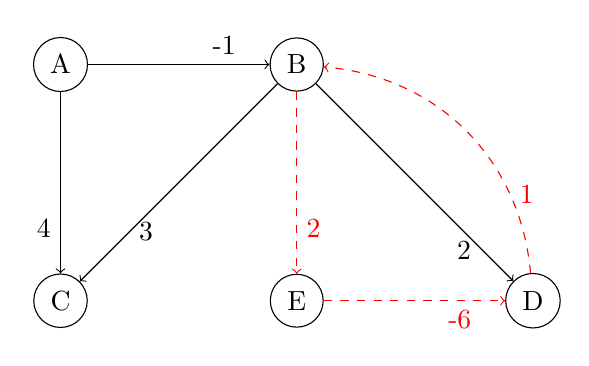
\begin{tikzpicture}
  \node[shape=circle,draw=black] (A) at (0,0) {A};
  \node[shape=circle,draw=black] (B) at (3,0) {B};
  \node[shape=circle,draw=black] (C) at (0,-3) {C};
  \node[shape=circle,draw=black] (E) at (3,-3) {E};
  \node[shape=circle,draw=black] (D) at (6,-3) {D};
  \path [->](A) edge node[near end,above] {-1} (B);
  \path [->](A) edge node[near end, left] {4} (C);
  \path [->](B) edge node[near end,right] {3} (C);
  \path [->](B) edge node[near end, below] {2} (D);
  \path [->,red,dashed](B) edge node[near end, right] {2} (E);
  \path [->,red,dashed](E) edge node[near end,below] {-6} (D);
  \path [->,red,dashed](D) edge[bend right=40] node[near start, right] {1} (B);
\end{tikzpicture}
